% Cover letter: Product Manager, strumenti interni Operations (payroll, contrattualistica, adempimenti), Jet
% CV: Sections/cv_product_manager_ops.tex -> cv_gen/cv_giovanni_tauro-jet.pdf
% Letter in Italian (the posting is in Italian). babel-italian is not installed here,
% so hyphenation is switched off instead of using English patterns on Italian words.
\documentclass[11pt,a4paper,sans]{moderncv}
% Shared preamble and header for the cover letters.
% One main file per application: cl_<company>.tex, built to
% cv_gen/coverletter_giovanni_tauro-<company>.pdf next to cv_giovanni_tauro-<company>.pdf.
% Paths (cl_gen/..., Pictures/...) are relative to the project root, as in the CV (see .latexmkrc).

\moderncvstyle{classic}
\moderncvcolor{blue}

\usepackage[scale=0.80]{geometry}
\setlength{\footskip}{136.00005pt}

\usepackage{fontawesome5}
% hyperref is loaded by moderncv itself; loading it here causes an option clash
\usepackage{xcolor}
\usepackage{graphicx}
\ifxetexorluatex
  \usepackage{fontspec}
  \usepackage{unicode-math}
  \defaultfontfeatures{Ligatures=TeX}
  \setmainfont{Latin Modern Roman}
  \setsansfont{Latin Modern Sans}
  \setmonofont{Latin Modern Mono}
  \setmathfont{Latin Modern Math}
\else
  \usepackage[T1]{fontenc}
  \usepackage{lmodern}
\fi

\usepackage[english]{babel}

% used for the PDF title and the letter closing; the visible header is \clheader below
\name{Giovanni}{Tauro}

% Header: #1 = headline under the name (same as the headline of the matching CV)
\newcommand{\clheader}[1]{%
\noindent
\begin{minipage}[c]{0.74\textwidth}
    {\Huge \textbf{Giovanni Tauro}}\\[-0.2em]
    {\small #1}\\[0.3em]

    \footnotesize
    \faMapMarker*~
    \href{https://www.google.com/maps/search/?api=1&query=Lecco+23900+Italy}
    {\color{blue}Bari-Lecco, Italy}
    \quad
    \faPhone*~
    \href{https://wa.me/393279437161}
    {\color{blue}+39 3279437161}
    \quad
    \faEnvelope~
    \href{mailto:giovanni.taurodi@gmail.com}
    {\color{blue}giovanni.taurodi@gmail.com}
    \\[-0.1em]

    \faLinkedin~
    \href{https://www.linkedin.com/in/giovanni-tauro-gt/}
    {\color{blue}LinkedIn}
    \quad
    \faGithub~
    \href{https://github.com/jotades}
    {\color{blue}GitHub}
    \quad
    \faGraduationCap~
    \href{https://scholar.google.com/citations?user=BS0aVGgAAAAJ&hl=it}
    {\color{blue}Scholar}
    \quad
    \faFilePdf~
    \href{https://www.notion.so/Giovanni-Tauro-2a7901d92f3a800b892af425c5875c6a}
    {\color{blue}Portfolio}
    \quad
    \faCubes~
    \href{https://grabcad.com/giovanni.tauro-3}
    {\color{blue}GrabCAD}

\end{minipage}
\hfill
\begin{minipage}[c]{0.18\textwidth}
    \raggedleft
    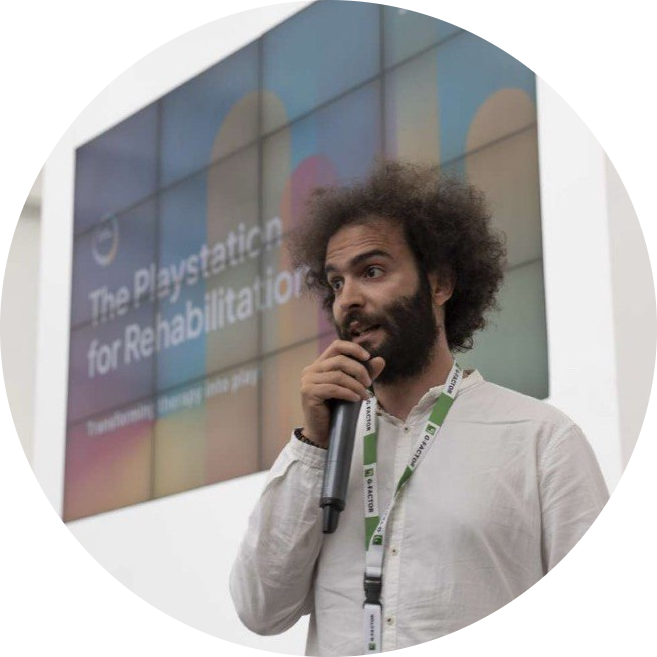
\includegraphics[width=2.8cm]{Pictures/Giovanni_pitch}
\end{minipage}
\vspace{0.1em}
}

\makeatletter
% the sender details are already in \clheader, so skip moderncv's own block
\@detailsfalse
% closing phrase, signature, name
\renewcommand*{\makeletterclosing}{%
  \@closing\\[0.6em]%
  
\includegraphics[height=1.2cm]{Pictures/sign_gt.jpg}\\[0.2em]%
  {\bfseries\@firstname~\@lastname}}
\makeatother


\begin{document}
\hyphenpenalty=10000 \exhyphenpenalty=10000 \emergencystretch=3em

\clheader{Head of Product | Internal Tools, Data \& Processes}

\recipient{Team Talent}{Jet}
\date{16 ottobre 2026}
\opening{Gentile team di selezione,}
\closing{Cordiali saluti,}
\makelettertitle

vi scrivo per candidarmi alla posizione di Product Manager sugli strumenti interni del team Operations. Sono Head of Product e co-fondatore di Rehabilia Technologies e da più di cinque anni lavoro in R\&D al CNR-STIIMA, sempre in un dominio regolamentato: i dispositivi medici.

Nell'annuncio la competenza più importante è mettere ordine, e il mio lavoro parte quasi sempre da lì. Con PhiCube, il dispositivo per la riabilitazione di cui sono co-inventore, ho raccolto con clinici e terapisti come lavoravano davvero, spesso in modo non documentato, e l'ho trasformato in requisiti e specifiche per l'ingegneria, tenendo insieme i vincoli normativi (MDR, ISO 13485, IEC 60601) e la documentazione tecnica per la marcatura CE. Oggi il dispositivo è usato in cliniche italiane, ha ottenuto 85,8/100 di usabilità (SUS) con 19 bambini ed è in due studi multicentrici con 134 pazienti.

Conosco bene anche lo strumento interno visto da chi lo costruisce. Per il mio dottorato ho progettato OmniAnalytics, uno strumento che trasforma le registrazioni grezze di uno studio con 16 partecipanti non vedenti in metriche standard. La parte più delicata non è stata il calcolo, ma le eccezioni: correzioni, esclusioni e annotazioni sono salvate a parte, così i dati originali non vengono mai modificati e ogni risultato si può ricostruire. Conosco abbastanza sistemi, database e integrazioni da discuterne con i developer.

In Rehabilia le richieste sono sempre più di quelle che possiamo sviluppare. Decido io cosa entra in ogni rilascio, usando i dati degli studi e il feedback degli utenti, e spiego a clinici, ingegneri e partner perché il resto aspetta.

Payroll e contrattualistica sono domini nuovi per me. Porto però l'abitudine a imparare in fretta un dominio specialistico accanto a chi lo vive ogni giorno, come ho fatto con i clinici, e a misurare una funzionalità da quello che cambia nel lavoro delle persone.

Sarei felice di raccontarvi di più in un colloquio.

\makeletterclosing

\end{document}
